\begin{sectionbox}{Propiedades básicas de las ondas: amplitud, longitud de onda y frecuencia}
Como tal vez ya sabrás, una onda tiene un valle (punto más bajo) y una cresta (punto más alto). La distancia vertical entre la punta de la cresta y el eje central de la onda se conoce como amplitud. Esta es la propiedad asociada con el brillo, o intensidad, de la onda. La distancia horizontal entre dos crestas o valles consecutivos de la onda se conoce como longitud de onda. Podemos visualizar estas longitudes de onda de la manera siguiente:

\begin{figure}[H]
    \centering
    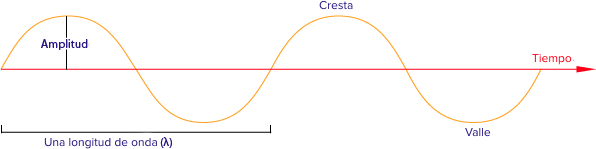
\includegraphics[width=0.7\linewidth]{../images/67a8bb901b1aae76df573aa510cf0ee6c6229496}
    \caption{Las características principales de una onda, incluyendo la amplitud y la longitud de onda.}
    \label{fig:67a8bb901b1aae76df573aa510cf0ee6c6229496}
\end{figure}

Ten en cuenta que algunas ondas (incluyendo las ondas electromagnéticas) también oscilan en el espacio, y por lo tanto oscilan en una posición dada conforme pasa el tiempo. La cantidad de la onda conocida como frecuencia describe el número de longitudes de onda completas que pasan por un punto dado del espacio en un segundo; la unidad del SI para la frecuencia es el hertz (hz) o (1/s).
Como te imaginarás, la longitud de onda y la frecuencia son inversamente proporcionales; es decir, mientras más corta sea la longitud de onda, más alta será la frecuencia, y viceversa. Esta relación está dada como se muestra a continuación:

\begin{multicols}{2}
    \include*{../blocks/block006b}
    \include*{../blocks/block006c}
\end{multicols}
\end{sectionbox}